\documentclass[..\EOYR.tex]{subfiles}

\begin{document}

\section{Background}
Tell a story up to where we are and what's missing.
\paragraph{Literature Review (take most from coursework).Cover the various angles including:}
\begin{itemize}
  \item Turbulence and bathymetry - understanding the smaller processes (vorticity etc.) \citep{Tansley2001} \citep{Nikurashin2012a}
  \item Inclulde some phenomenology - e.g. bottom vortex stretching and bottom pressure torque. Maybe also the weird sandwhich diagram!
  \item Include context of climate modelling (e.g. Scaife et al, Ezer summary etc)
  \item context of what affects the Gulf Stream etc.
  \item Possible relationships/data sets to see the history of the Gulf Stream. (Palaeo?) \citep{Ezer2015}
  \item Cut down lit review - parts of it will be elsewhere!! (or should be! OR Remove them from elsewhere to keep them here!!)
  \item When introducing equations... maybe start with the basic equations then the vector invariant form of the momentum equation etc...????
  \item Modelling \& vertical grid systems - include partial cells
  \item Balance between acceleration by wind stress and decelleration by pressure force on bottom topography \citep{NaveiraGarabato2013} - he cites Vallis 2006 (Geoff's book!)??
\end{itemize}

\td{Do I need to introduce the background? Do I have it as a lit review? Or Split it into separate topics within my thingy???? WAAAAAAAAAAAH}

\subsection{Gulf Stream Separation \& NAC}
\begin{itemize}
    \item Maybe lead in through the Gulf Stream intro?
    \item Frame it in ocean eddies etc and energy transfer?
\end{itemize}

The Gulf stream separates at Cape Hatteras, skirts the Grand Banks at Newfoundland and then heads Eastwards towards western Europe. However, in many moderate resolution climate models this separation occurs further north than observed and turns more sharply to the East, as noted in \citep{Hurlburt2008} and often misses off the Grand Banks, heading straight towards Europe. This can lead to what modellers refer to as the "blue spot of death" \citep{Gnanadesikan2007}, a patch of colder than observed SSTs resulting from the lack of heat at Newfoundland normally brought up by the Gulf Stream.

The exact cause for the path of the Gulf Stream is unknown, though it has been a research topic for many years and is still a popular topic amongst researchers today. A recurring theme when looking into the separation of the Gulf Stream is the mention of bathymetry. It is thought \citep{Gula2014}\citep{NaveiraGarabato2013}\citep{Nikurashin2012a} that the ocean dynamics resulting from the interaction of the Gulf Stream and the deep western boundary current (DWBC) with the bathymetry in the North Atlantic could cause the turbulence required to direct the Gulf Stream along its path. A sudden change in the direction of the Gulf Stream just off the coast at South Carolina and Georgia has been attributed to the Charleston Bump, a topographical feature which raises the ocean floor, from a depth of 600m on the surrounding Blake Plateua to 200m \citep{Gula2014}. Hence it is clear that bathymetry can strongly impact the direction of ocean currents.


\subsection{Subpolar Gyre \& subtropical gyre?}

\subsection{The Effects of topography}
\begin{itemize}
    \item Maybe introduct Streamfunction?
    \item Include Bottom Pressure Torque
    \item Include JEBAR
    \item Include Vortex Stretching etc. \citep{Zhang2007}
    \item \citep{Bell1999}
    \item Bottom Pressure Torque to JEBAR. JEBAR is part of bottom pressure torque (see Geoff's book \& \citep{Greatbatch1991}). The additional term corresponds to the torque of the vertically averaged pressure (\citep{Greatbatch1991})
\end{itemize}

The horizontal components of the vector invariant form of the momentum equation are: (From Geoff's book P64)
\begin{equation}\label{VIMomentumU}
    \frac{\partial u}{\partial t} - (f+\zeta)v + w\frac{\partial u}{\partial z} = -\frac{1}{a cos \phi}(\frac{1}{\rho}\frac{\partial p}{\partial \lambda} + \frac{1}{2}\frac{\partial \mathbf{u}^2}{\partial \lambda})
\end{equation}
and
\begin{equation}\label{VIMomentumV}
    \frac{\partial v}{\partial t} - (f+\zeta)u + w\frac{\partial v}{\partial z} = -\frac{1}{a}(\frac{1}{\rho}\frac{\partial p}{\partial \phi} + \frac{1}{2}\frac{\partial \mathbf{u}^2}{\partial \phi})
\end{equation}

We start with the primitive horizontal momentum equations in spherical coordinates:
\td{Primitive: 3 approximations: (From Geoff's book)}
\begin{itemize}
    \item The hydrostatic approximation. In the vertical momentum equation the gravitational term is assumed to be balanced by the pressure gradient term, so that
        \begin{equation}
            \frac{\partial p}{\partial z} = -\rho g
        \end{equation}
        The advection of vertical veloicyt, the coriolis terms and the metric term $\frac{(u^2 + v^2)}{r}$ are all neglected.
    \item The shallow-fluid approximation. We write $r=a+z$ where the constant $a$ is the radius of hte Earth and $z$ increases in the radial direction. The coordinate $r$ is hten replaced by $a$ except where it is used as the differentiating argument. Thus, for example,
        \begin{equation}
            \frac{1}{r^2}\frac{\partial (r^2 w)}{\partial r} \to \frac{\partial w}{\partial z}
        \end{equation}
    \item The traditional approximation. Coriolis terms in the horizontal momentum equations involving the vertical velocity, and the still smaller metric terms $uw/r$ and $vw/r$, are neglected.
\end{itemize}

Then the governing equations become:
\begin{equation} \label{PrimMomUMB}
    \frac{\partial u}{\partial t}=-((\mathbf{u}.\nabla)u - \frac{uv\tan \phi }{a}) + fv - \frac{1}{\rho_0 a \cos \phi}\frac{\partial p}{\partial \lambda} + \frac{1}{\rho_0}\frac{\partial \tau_\lambda}{\partial z} + F_\lambda
\end{equation}
\begin{equation} \label{PrimMomVMB}
    \frac{\partial v}{\partial t}=-((\mathbf{u}.\nabla)v + \frac{u^2\tan \phi }{a}) - fu - \frac{1}{\rho_0 a}\frac{\partial p}{\partial \phi} + \frac{1}{\rho_0}\frac{\partial \tau_\phi}{\partial z} + F_\phi
\end{equation}

\td{Find a way to label the terms as nonlinear advection, coriolis acceleration, pressure gradient force, vertical diffusion of momentum, and horizontal diffusion of momentum.}\textcolor{magenta}{Maybe find an eqn with the 7 terms I'm using instead!?! have found the 7 terms in nemo - maybe work with this for now and come back to it later.}

\ignore{\begin{equation} \label{PrimMomUGV}
    \frac{\partial u}{\partial t}=2\Omega\sin\phi v - (\mathbf{u}.\nabla)u + \frac{uv\tan \phi }{a} - \frac{1}{\rho_0 a \cos \phi}\frac{\partial p}{\partial \lambda}
\end{equation}
\begin{equation} \label{PrimMomVGV}
    \frac{\partial v}{\partial t}=-2\Omega\sin\phi u - (\mathbf{u}.\nabla)v - \frac{u^2\tan \phi }{a} - \frac{1}{\rho_0 a}\frac{\partial p}{\partial \phi}
\end{equation}}


\td{Make sure to define $\phi$ as going from the equator!!! and $\lambda$ as the azimuth}



\subsubsection*{Bottom Pressure Torque}
\td{JUST NOTES}
\citep{Greatbatch1991} Fig 1 \& Fig 5 differences show the effect of bottom pressure torque missing from models which assume a flat bottom. They then have equations to demonstrate ((16) \& (17)). \citep{Greatbatch1991} say bpt forcing responsible for enhacnign max transport of the subtropical gyre which combined with significant bpt forcing to the SE of the Grand Banks is important for determining the max trasnport of the diagnosed gulf stram. \\
\td{See notes on Greatbatch paper in Papers doc for eqns - rewrite these in more modern notation - maybe consult Geoff's book!}
\citep{Yeager2015} "The relationship between JEBAR and BPT has been clarified by, among others, Mertz and Wright (1992), Greatbatch et al. (1991), and Bell (1999); the former arises in the (potential) vorticity equation of the vertically averaged horizontal flow, whereas the latter arises in the vorticity equation of the vertically integrated horizontal flow (see appendixA). JEBAR represents the component of BPT associated with the baroclinic (buoyancy de- pendent) part of the pressure gradient, and therefore it vanishes in the absence of stratification (Mertz andWright 1992; Salmon 1998). BPT can be nonzero regardless of stratification because it represents the projection of hori- zontal geostrophic bottom flow normal to isobaths. With the condition of no normal flowat the ocean bottom,BPT can be understood as a geostrophic bottom vortex stretching" (See eq (1) in paper).

We start with the \td{blah blah} of the momentum equation,
\begin{equation}\label{momentum}
\end{equation}

\subsubsection*{JEBAR}
\td{JUST NOTES}
\citep{Greatbatch1991} JEBAR accounts for part of the bottom pressure torque - Greatbatch has a good example of difference between solutions where JEBAR is 0 and other part is 0 to show the significance of JEBAR term.

Then JEBAR itself can be split into separate parst - see \citep{Greatbatch1991} and \citep{Gula2014}.\\

\td{See notes on Greatbatch paper in Papers doc for eqns - rewrite these in more modern notation - maybe consult Geoff's book!}


The Joine Effect of Baroclinicity And Relief (JEBAR) was first introducted to account for the effects of topography and baroclinicity in ocean dynamics. It is these effects which balance with the wind stress. This is terrible writing oh my god what areyou doing. just write something half way decent. In fact just write anything. Find an equation to write down to explain what JEBAR is.

\subsubsection*{Bototm Vortex Stretching}

\subsection{Small Scale Processes}
\begin{itemize}
    \item Lots from lit review - and add some dissipation stuff.
\end{itemize}


It has been noted that in higher resolution models, the separation and subsequent path of the Gulf Stream is much more accurate than in the lower resolution counterparts \citep{Hurlburt2008}\citep{Zhang2007}. This lends to the idea that the processes which affect the Gulf Stream occur on smaller scales which aren't resolved by coarser models \citep{NaveiraGarabato2013}\citep{Nikurashin2012a}. Various processes have been investigated and suggested as the main influences though it is likely that the improved Gulf Stream representation is due to multiple factors.


\citep{NaveiraGarabato2013} theorised that interaction with the bathymetry creates small-scale turbulence and instabilities which could cause bathymetric steering and divert currents. If this is not being represented in coarser models, the energy behind the turbulence must be going elsewhere. \citep{Scott2010} compared current meter readings with modelled values for kinetic energy and noticed that in some areas of the North Atlantic the total kinetic energy was being held higher in models than observed. It is discrepancies such as this which could have much wider implications. If the energy is not penetrating to the ocean floor, we cannot expect to be able to replicate the effects of the bathymetry. Perhaps by pulling this energy further down (closer to observed values), there would be more energy transfer from the larger ocean eddies to the smaller scale turbulence resulting from interaction with the bathymetry.

\citep{Tansley2001} used a simplified model of water flowing past a cylinder to highlight the importance of turbulence on fluid motion. Using a quarter-cylinder ( mimicking a simplified version of Cape Hatteras) and a high Reynolds number (allowing for more turbulent flow), the model produced a jet with surrounding turbulent eddies similar to those observed in the Gulf Stream. These results were not seen with a lower Reynolds number, highlighting the importance of turbulence in forming jets like the Gulf Stream.

The turbulent mixing arising from interaction with the bathymetry could allow geostrophic eddies to transfer some of their energy to smaller processes by causing internal waves to break and contribute to enhanced mixing \citep{Nikurashin2012a}. These effects have been seen even in cases of small-scale bathymetric roughness suggesting that it is not necessary to have large topological features to impact ocean dynamics, instead small surface differences can cause changes which lead to bigger outcomes.

\citep{NaveiraGarabato2013} attribute the significant impact of small-scale bathymetry to wave drag. Although wave drag is not a large contributor to ocean dynamics, topological features on a small scales can cause wave drag which contributes ten to several tens of a percentage of the dominant source and sink terms influencing the vorticity of the ocean.


These effects of small-scale processes are not limited to the Gulf Stream, but impact on many aspects of ocean dynamics as the various currents and features affect one another. 
\citep{Ezer2016} speculated that amongst other things, the northern branches of the Northern Recirculation Gyre (NRG) would have to be resolved in order to produce an accurate Gulf Stream in a model. \citep{Zhang2007} determined that a significant contribution to the generation of the NRG is the bottom vortex stretching resulting from a downslope DWBC, which is in turn the result of the interaction with bathymetry as the DWBC crosses the path of the Gulf Stream. Hence, bathymetric impact can circle around to affect many aspects of ocean dynamics.


\subsection{Energy Dissipation}
\begin{itemize}
    \item How the energy is changed from global eddies to smaller spin and/or lost. internal wave drag etc?
\end{itemize}

\subsection{Climate Models}
\begin{itemize}
    \item Talk about model resolution and improvements
    \item Mention Zanna paper???
    \item Different vertical coordinate systems
    \item Effects of the Gulf Stream in models etc. Scaife et al...
    \item Parameterisations and improvements etc. Work being done on the more modelly side!
\end{itemize}

\paragraph{Modelling the Gulf Stream}

As more scientists seek to understand ocean dynamics, more models are made and used by different researchers to simulate different processes. There are many models in use today, all with different configurations and settings. This can lead to contrasting outcomes and debate over which choice of model or model settings yields the most accurate results.

\paragraph{Model Resolution}

\subparagraph
	Along with differing numerical schemes or boundary conditions, etc. there are also many different model resolutions available. These range from coarse 1$\degree$ models, which resolve to a scale of $\approx$ 100km, to higher resolution 0.25$\degree$ models, which resolve to a scale of $\approx$ 25km, all with varying numbers of vertical levels. It is well established \citep{Scaife2011a}\citep{Hurlburt2008} that a higher resolution ocean model tends to produce a more accurately resolved Gulf Stream. This is in part due to the small scale processes, mentioned previously, which contribute to the ocean circulation, but are not resolved in the coarser models. Unfortunately higher resolution models require additional processing power and thus additional costs. This means that the high resolutions required to resolve a realistic Gulf Stream will not be widely used for some time. Hence, the aim is to find a way to represent an accurate Gulf Stream in the lower resolution models by understanding the reasons behind it.

\paragraph{Vertical Coordinate System}

\subparagraph
	One of the main variabilities between different models is the handling of the vertical coordinate system. The way in which the model splits the depth of the ocean into 'levels' can have a large impact on the way the bathymetry is represented. As previously discussed, this bathymetric representation can have large impacts on the dynamics within the model. The importance and significance of the bathymetric roughness has already been discussed in this review so it is now necessary to discuss the different ways to represent this.
\subparagraph
The main coordinate systems in use are the z-coordinate system which stays true to a cartesian system of coordinates, consisting of rectangular 'blocks', which create a staircase effect when representing slopes. These z-coordinate systems can also be implemented with 'partial cells' whereby some of the cells are cut into smaller cells to 'smooth out' and more closely represent the shape of the slopes. Thre are also s- (or sigma-) coordinates which follow the shape of the terrain. The depth at any point is divided by the number of levels to create a consistent number of cells at all points of different thickness. These different approaches can also be combined to form hybrid coordinate systems. See Figure \ref{fig:coords} for an illustration of some of the possible vertical coordinate systems available in the NEMO model.

\begin{figure}
  \centering
  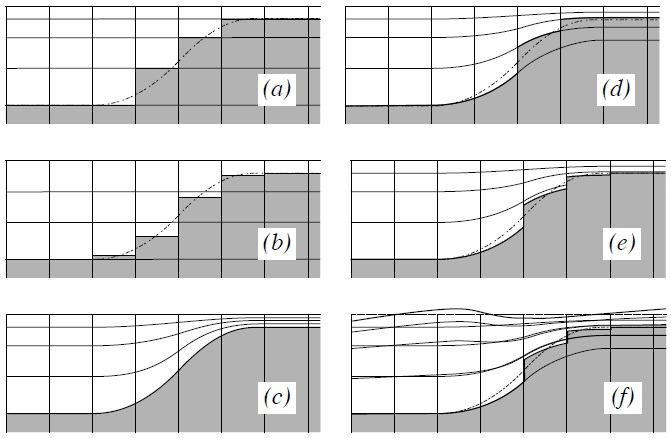
\includegraphics[scale=.8]{NEMOP58.jpg}
  \caption{An illustration of different veritcal coordinate systems available in NEMO. \citep{Madec2011}. (a) z-coordinate, (b) z-coordinate with partial cells, (c) s-coordinate, (d) hybrid s-z coordinate, (e) hybrid s-z coordinate with partial cell, (f) shows (e) with a non-linear free surface (which can be used with any coordinate system).}
  \label{fig:coords}
\end{figure}

\subparagraph
The main difficulty in comparing different vertical coordinate systems lies in the availability of a 'control' case for the comparison. With the wide selection of models available to researchers, it is not only the vertical coordinate system which differs but also the numerical schemes being used to resolve various processes. This could lead to false similarities or differences and cause incorrect conclusions. \citep{Ezer2016} was able to compare results from z-coordinate models and s-coordinate models while minimalising any other differnces between the models. Although the z-coordinate models are capable of producing an accurate Gulf Stream at hight resolutions, the s-coordinate models provided a more accurate representation when restricted with coarser models. However, as \citep{Ezer2016} noted in the comparison, partial and shaved cells (whereby corners of the cells are 'shaved' off to smooth out slopes) were not used in any of these models.




\end{document}
